\documentclass[a4paper, twocolumn, 12pt]{article}
\XeTeXlinebreaklocale "zh"
\XeTeXlinebreakskip = 0pt plus 1pt
\usepackage{fontspec}
\usepackage{geometry}
\usepackage{graphicx}
\usepackage{indentfirst}
\usepackage[colorlinks, linkcolor=blue]{hyperref}

\geometry{left=2.5cm,right=2.5cm,top=1.0cm,bottom=2.5cm}
\setmainfont{思源宋体 CN}

\title{\huge {朴素贝叶斯文本分类器}\\[1ex]\small Artificial Intelligence Course, Fall 2017}

\author{
    张义飞\\2014000201010
    \and 周峙龙\\2014000201004
    \and 冯齐\\2014000202000
}

\date{\today}

\begin{document}
\maketitle

\section{摘要}

在人们的日常生活中,垃圾邮件常常影响人们的心情和工作效率。例如,人们会因为阅读一篇垃圾邮件而浪费时间和精力。所以,分类垃圾邮件一直是一个贴近生活并且有很大作用的应用。\\

分类垃圾邮件,这是一个二分类问题,在机器学习中有很多分类器能够用来解决这样一个二分类问题,例如支持向量机(SVM),朴素贝叶斯分类器等。在这次设计中,我们使用朴素贝叶斯分类器来分类垃圾邮件。\\

在机器学习中,朴素贝叶斯分类器是一系列以假设特征之间强(朴素)独立下运用贝叶斯定理为基础的简单概率分类器。\\

朴素贝叶斯是一种构建分类器的简单方法。该分类器模型会给问题实例分配用特征值表示的类标签,类标签取自有限集合。它不是训练这种分类器的单一算法,而是一系列基于相同原理的算法:所有朴素贝叶斯分类器都假定样本每个特征与其他特征都不相关。举个例子,如果一种水果其具有红,圆,直径大概3英寸等特征,该水果可以被判定为是苹果。尽管这些特征相互依赖或者有些特征由其他特征决定,然而朴素贝叶斯分类器认为这些属性在判定该水果是否为苹果的概率分布上独立的。\\

对于某些类型的概率模型,在监督式学习的样本集中能获取得非常好的分类效果。在许多实际应用中,朴素贝叶斯模型参数估计使用最大似然估计方法;换而言之,在不用到贝叶斯概率或者任何贝叶斯模型的情况下,朴素贝叶斯模型也能奏效。\\

朴素贝叶斯自20世纪50年代已广泛研究。在20世纪60年代初就以另外一个名称引入到文本信息检索界中,并仍然是文本分类的一种热门(基准)方法,文本分类是以词频为特征判断文件所属类别或其他(如垃圾邮件、合法性、体育或政治等等)的问题。通过适当的预处理,它可以与这个领域更先进的方法(包括支持向量机)相竞争。它在自动医疗诊断中也有应用。\\

在本文中,我们使用朴素贝叶斯方法来实现文本分类进而分类垃圾短信。我们的训练集是由5574条短信构成,其中有747条垃圾短信。我们使用了交叉验证的方法对我们的分类器进行了验证,最后得到了很好的结果。\\

本文的结构如下:在第2部分,我们将介绍朴素贝叶斯的基本原理以及我们实现的思路。在第三部分,我们展示我们分类器所得到的结果。在第四部分,我们对这次的课程设计做一个总结。

\section{主要方法}
\subsection{朴素贝叶斯概率模型}
理论上,概率模型分类器是一个条件概率模型:
\[ P(C|F_1, ..., F_n) \]
独立的类别变量$C$有若干类别,并且条件依赖于若干特征变量$F_1, F_2, ..., F_n$。\\

在此之前,我们先引入贝叶斯定理(Bayes theorem),对于互相独立的事件集合${B_1, B_2, ..., B_n}$,满足条件$\sum_{i=1}^n P(B_i)=1$,则对于事件$A$有:
\[P(B_i|A)=\frac{P(B_i)P(A|B_i)}{\sum_{i=1}^n P(B_i)P(A|B_i)}\]
通过贝叶斯公式,我们可以由独立事件集合的先验概率(Prior probability)来计算相应事件的后验概率(Posterior probability)。\\

在朴素贝叶斯概率模型中,贝叶斯表现如下:
\[P(C|F_1, ..., F_n)=\frac{P(C)P(F_1, ..., F_n|C)}{P(F, ..., F_n)}\]
实际上,我们只需关心式子的分子部分,因为分母并不依赖于$C$,并且特征$F_i$的值是给定的,即分母是一个常数。\\

朴素贝叶斯假设各个特征是相互独立的,即:
\[P(F_i|C, F_j)=P(F_i|C), j \neq i\]
根据这一假设,我们可以对分子进行分解,即:
\[P(F_1, ..., F_n|C)=\prod_{i=1}^nP(F_i|C)\]
然后,我们就得到了独立分布特征模型:
\[P(C|F_1, ..., F_n)=\frac{P(C)\prod_{i=1}^n P(F_i|C)}{P(F_1, ..., F_n)}\]
\subsection{构造分类器}
由以上推导出的独立特征模型,我们可以构造相应的分类器,也就是朴素贝叶斯分类器。朴素贝叶斯分类器采用最大后验概率作为决策规则,及对于各个类别$C_i$,取后验概率最大的类别作为选定类别。每个类别的后验概率计算公式为:
\[P(C_i|F_1, ..., F_n)=\frac{P(C_i)\prod_{j=1}^nP(F_j|C)}{\sum_{i=1}^m \prod_{j=1}^nP(C_j)P(C_j|F_k)}\]

\subsection{使用互信息筛选特征词}
直接用训练集中所有出现过的词汇做为特征词汇,会导致分类器的词表十分巨大,从而降低算法的性能。因此,我们决定提取其中的部分词汇,做为特征词。\\

理想的特征词应当与分类结果密切相关。在概率论和信息论中,两个随机变量的互信息(Mutual Information,简称MI)是变量间相互依赖性的量度。一般地,两个随机变量$X, Y$的互信息可以定义为:
\[MI(X; Y)=\sum_{y\in Y}\sum_{x\in X}p(x, y)log(\frac{p(x, y)}{p(x)p(y)})\]
其中$p(x,y)$是$X$和$Y$的联合概率分布函数,而$p(x)$和$p(y)$分别是$X$和$Y$的边缘概率分布函数。\\

我们计算了所有在训练集中出现的词汇与词汇所在类别的互信息,然后按照互信息值的大小排序,选取前n个词汇作为特征词,从而使算法的复杂度大幅度降低。

\begin{table*}[hbtp]
    \centering
    \caption{SMS Spam Collection 数据集部分样本}
    \begin{tabular}{lp{14cm}}
        \hline
        ham&	Go until jurong point, crazy.. Available only in bugis n great world la e buffet... Cine there got amore wat...\\
        ham&	Ok lar... Joking wif u oni...\\
        spam&	Free entry in 2 a wkly comp to win FA Cup final tkts 21st May 2005. Text FA to 87121 to receive entry question(std txt rate)T\&C's apply 08452810075over18's\\
        ham&	U dun say so early hor... U c already then say...\\
        ham&	Nah I don't think he goes to usf, he lives around here though\\
        \hline
    \end{tabular}
    \end{table*}

\section{实验结果}
我们使用了一个公开的骚扰短信标注数据集(SMS Spam Collection v.1, \url{http://www.dt.fee.unicamp.br/~tiago/smsspamcollection/})进行训练,该数据集包含了5574条英文短信数据,其中骚扰短信有470条,正常短信为4827条。\\
[2ex]
\begin{figure*}
    \centering
    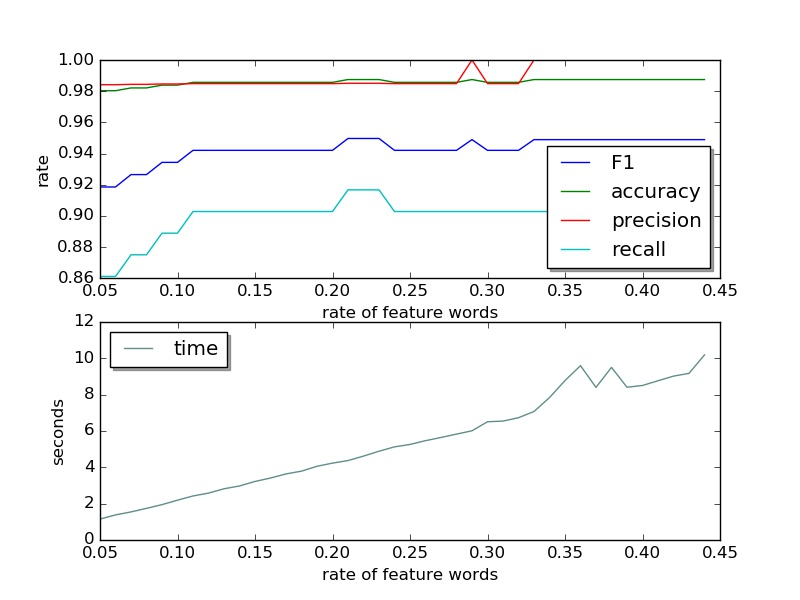
\includegraphics[width=0.8\textwidth]{fig_1.jpg}
    \caption{与sklearn中的分类器的性能对比}
\end{figure*}
\end{document}